\begin{frame}
	\frametitle{Filtros digitais \textit{wavelet}}
	\only<1>{
		\framesubtitle{Propriedades}
		\begin{itemize}
			\item Suporte compacto.
			\item Análise multirresolução.
			\item Wavelet regular e wavelet packet.
			\item Análise detalhada em altas e baixas frequências.
		\end{itemize}
	}
	\only<2>{
		\framesubtitle{Restrição de escopo}
		\begin{itemize}
			\item Domínio discreto.
			\item Apenas transformadas diretas.
			\item Não haverá reconstrução do sinal.
			\item Construção dos vetores de características.
		\end{itemize}
	}

	\only<3>{
		\framesubtitle{Resposta em frequência e linearidade}
		\begin{table}[h]
	\centering
	\caption{Algumas das \textit{wavelets} mais usadas e suas propriedades}
	\begin{tabular}{|c|p{75mm}|c|}
			\hline 
			\textbf{Wavelet} & \textbf{Resposta em frequência} & \textbf{Resposta em fase} \\ 
			\hline 
			Haar & Pobre &  Linear \\ 
			\hline 
			Daubechies & mais próxima da ideal à medida que o \newline  suporte aumenta; \textit{maximally-flat}  &  Não linear \\ 
			\hline 
			Symmlets & mais próxima da ideal à medida que o \newline  suporte aumenta; não \textit{maximally-flat}  & Quase linear \\ 
			\hline 
			Coiflets & mais próxima da ideal à medida que o \newline  suporte aumenta; não \textit{maximally-flat}  & Quase linear \\ 
			\hline 
	\end{tabular} 
	\label{tab:waveletsProperties}
	\\Fonte: Elaborado pelo autor, 2022.
\end{table}

	}

	\only<4>{
		\framesubtitle{Algoritmo de Malat}
		\begin{itemize}
			\item \textit{Wavelet} Haar: $h[\cdot] = [\frac{1}{\sqrt{2}}, \frac{1}{\sqrt{2}}]$.
			\item Par ortogonal: $g[\cdot] = [\frac{1}{\sqrt{2}}, \frac{-1}{\sqrt{2}}]$.
			\item sinal: $s[\cdot] = [1,2,3,4]$.
		\end{itemize}
		
		\begin{equation*}
			\begin{pmatrix}
			\frac{1}{\sqrt{2}}, \frac{1}{\sqrt{2}}, 0, 0\\
			\frac{1}{\sqrt{2}}, \frac{-1}{\sqrt{2}}, 0, 0\\
			0, 0, \frac{1}{\sqrt{2}}, \frac{1}{\sqrt{2}}\\
			0, 0, \frac{1}{\sqrt{2}}, \frac{1}{\sqrt{2}}\\
			\end{pmatrix} 
			\cdot
			\begin{pmatrix}
			1\\
			2\\
			3\\
			4\\
			\end{pmatrix} 
			=
			\begin{pmatrix}
			\frac{3}{\sqrt{2}}\\
			\frac{-1}{\sqrt{2}}\\
			\frac{7}{\sqrt{2}}\\
			\frac{-1}{\sqrt{2}}\\
			\end{pmatrix}
			\Rightarrow \Big[
			\frac{3}{\sqrt{2}},
			\frac{7}{\sqrt{2}},
			\frac{-1}{\sqrt{2}},
			\frac{-1}{\sqrt{2}}
			\Big]\qquad.
		\end{equation*}
	}

	\only<5>{
		\framesubtitle{Exemplo de wavelet regular e packet}
		\begin{figure}
			\centering
			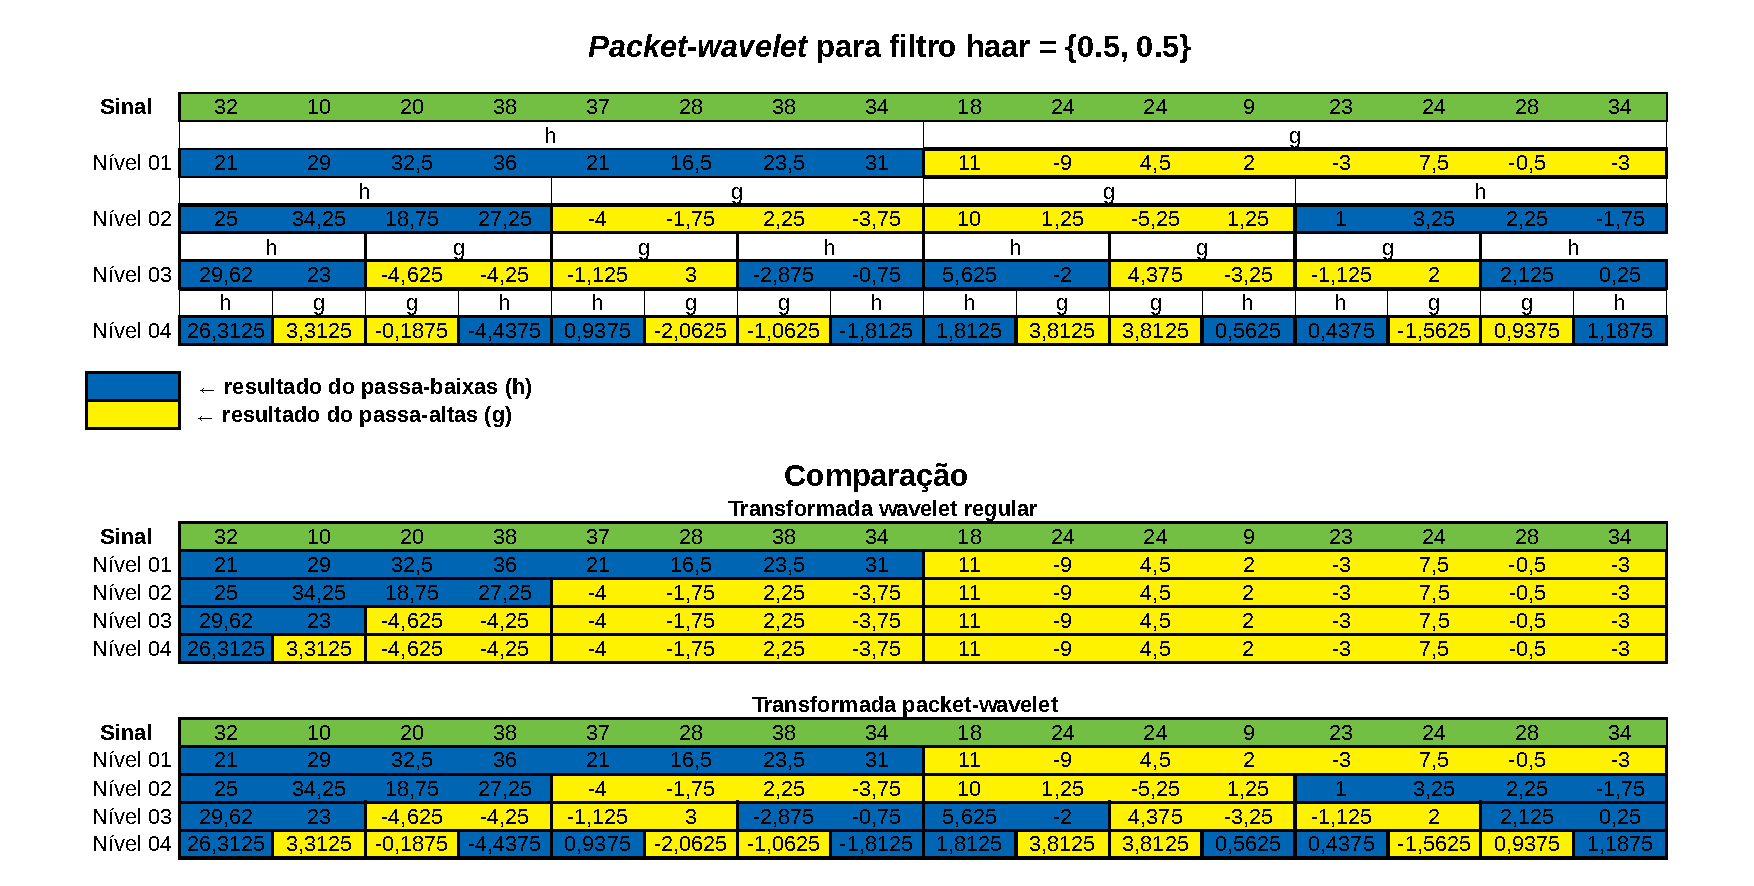
\includegraphics[width=\linewidth]{../monography/images/haarWaveletExamples}
		\end{figure}
	}
\end{frame}







